\documentclass{report}


\usepackage{biblatex}
\addbibresource{../../../Resources/resources.bib}

\usepackage{graphicx}
\usepackage{tikz}
\usetikzlibrary{arrows}
\usetikzlibrary{quantikz}

\usepackage{physics}
\usepackage{amsthm}
\usepackage{amsfonts}

\newtheorem{definition}{Definition}
\newtheorem{theorem}{Theorem}
\newtheorem{problem}{Problem}
\def\F{\mathcal{F}}

\title{Compiling Local Hamiltonians}
\author{Seyed Sajad Kahani \\ 22222815 \\Supervisor: Prof. Dan Browne}
\date{\today}
\begin{document}
\maketitle

\tableofcontents

\begin{abstract}
  This is a review essay that discusses the importance of local Hamiltonians in NISQ algorithms and the value of a compiler for them. The essay covers the basic concepts relevant to Hamiltonian compilation, including the Suzuki-Trotter formula, and examines the state-of-the-art methods in general quantum compilation. A structural approach is taken to explore the problems and algorithms associated with local Hamiltonian compilation. Finally, the essay discusses the open problems that will be addressed in the project, including possible ideas for extending gate set as well as improving scheduling.
\end{abstract}

\chapter{Introduction}

Quantum computation is an emerging field that aims to use quantum mechanics to solve problems that are intractable for classical computers. Since the earliest conceptualization of quantum computation~\cite{feynman1986}, it has been believed that quantum computers could revolutionize the way we solve problems, particularly those involving simulating nature. Over time, it has become clear that quantum computers have applications far beyond physical simulations. There are algorithms for search and traversing graphs, solving linear equations~\cite{montanaro2016}, and methods for machine learning and optimization~\cite{jordan2023}.

Despite significant efforts, we are still far from fully utilizing these algorithms. Our current hardware technology has not yet achieved the desired accuracy and number of qubits necessary for quantum computers to outperform classical computers in solving useful problems. This situation is commonly referred to as the ``noisy intermediate scale quantum'' (NISQ) era. In this era, the main barriers to run a general quantum algorithm are the effects of noise (especially for entangling gates) and decoherence time, which limits the depth of the circuit~\cite{preskill2018}.

Nevertheless, it is believed that some algorithms can still produce valuable results on NISQ devices. Quantum Variational Algorithms~\cite{cerezo2021}, as well as some simulation algorithms, are promising candidates for this purpose~\cite{preskill2018, langione2019}. Therefore, a problem-specific approach to quantum computation would be beneficial in the short-term.

Even for these promising candidates, circuit optimization is necessary~\cite{childs2018,farhi2016}. This raises the need for a specific-purpose quantum compiler. Moreover, while local Hamiltonians are commonly used in NISQ-era algorithms\cite{daley2022}, a compiler for them would be a valuable tool.

This project aims to improve existing methods for compiling local Hamiltonians, and this essay will focus on the literature review of these existing methods.

Various topics ranging from classical compilation to quantum information theory are not directly related to quantum compilers but are still beneficial in this study. These topics will be covered in chapter~\ref{chap:basic_concepts}. In chapter~\ref{chap:related_works}, we will review the literature on quantum compilers, as well as the state-of-the-art methods in the quantum compilation of local Hamiltonians. Chapter~\ref{chap:open_problems} will discuss the open problems that will be addressed in the project itself. Finally, we will conclude the essay in chapter~\ref{chap:conclusion}.
\chapter{Basic Concepts}\label{chap:basic_concepts}

\section{Classical Compilation}
A detailed study of the principles and heritage of classical compilers could be insightful and influential for any research conducted in the quantum compilation area. Rather than focusing on state-of-the-art results in classical compilation, we will focus on well-established principles to share the experience of classical compilers with quantum compilers.

In the context of executing computer programs, there are two main approaches: interpretation and compilation. Interpretation is the process of processing a program at the time of execution. It means that the processor of the program is aware of the input and the execution environment as well. While compilation refers to the process of transforming a program into another representation before the execution time, so the input and environment are not known at the moment~\cite[p. 2]{aho1986}.

For the quantum case, the transformation of programs (that are represented as gates) will be done before the execution, and the situation is quite similar to classical compilation. We can also assume the possibility of quantum interpretation, which is beyond our scope~\cite{gay2009}.

The process of compilation can be divided into three main phases:

\begin{itemize}
  \item \textbf{Parsing}: Using lexical and syntactic analysis, the source code is transformed into an abstract syntax tree (AST).

  \item \textbf{Intermediate Code Generation}: The AST is transformed into an intermediate representation (IR), which is a lower-level representation that is still device-independent. Any device-independent optimization will also take place here.

  \item \textbf{Target Code Generation}: The IR is transformed into the target code, which is the final representation of the program. The target code is device-dependent, and it is the final representation of the program.
\end{itemize}

Because of the common representation of quantum programs, a quantum compiler will never tackle the parsing phase, while the next two phases could be useful as a guideline for a quantum compiler.

Yet, the influence of classical compilers on quantum compilers may not be limited to the breakdown structure of the compilation process. They will also share some similar subproblems that we define as follows.

\begin{problem}[Register Allocation]
  \label{ref:register_allocation}
  Registers are the fastest memory in a computer. However, they are limited in number and size. Therefore, the compiler must decide at each time which variables should be stored in registers and which should be stored in memory.~\cite[pp. 440-444]{allen2001}
\end{problem}

\begin{problem}[Instruction Scheduling]
  There are some degrees of freedom regarding the order of instructions in a program. The compiler must decide which order is best for the program.~\cite[chap. 10]{allen2001}
\end{problem}

\begin{problem}[Code Motion]
  Code motion is the process of moving code to a different location in the program. This process may result in changes in the code snippets that are moved, but it will not change the semantics of the whole program. The compiler can move code to different locations to improve the performance of the program.~\cite[p. 592]{aho1986}
\end{problem}

\section{Quantum Computation}

Quantum computation could be defined using different models, such as quantum lambda calculus or quantum Turing machines. However, the most common model is the quantum circuit model, which is a model that is based on the quantum circuit model of quantum mechanics. In this model, a quantum computer is a quantum system that is prepared in a specific state, namely a state of $n$ qubits, that are typically in a basic product state. Then a sequence of quantum gates could be applied on any subset of qubits. By applying a quantum gate localy, we mean applying the indentity on the rest of the qubits. Finally, the state of the qubits is measured, and the result is the output of the quantum computer.

Now we will study a few more tools that are useful for our study.

One set of these tools is Decompositions of unitaries. They could be considered as a form of compilations as they transform a gate into a sequence of gates that are often simpler.

\section{Suzuki-Trotter Decomposition}

The Suzuki-Trotter decomposition~\cite{trotter1959, suzuki1991} is one of the most important tools for dealing with Hamiltonians. This decomposition approximates the time evolution of a Hamiltonian with a sequence of time evolutions of simpler Hamiltonians (terms of the first Hamiltonian). The simplest case is called the Lie-Trotter formula, and it is stated as follows.

\begin{theorem}[Lie Trotter Formula]
For any $H = A + B$,
\begin{equation}
  e^{iH} = \lim_{n \to \infty} (e^{iA/n} e^{iB/n})^n.
\end{equation}
\end{theorem}

Generally, the decomposition is stated as follows.
\begin{theorem}[Higher Order Suzuki-Trotter Decomposition]
  For any $H = \sum_{j=1}^k h_j$, we can define a series of approximations called $\tilde{U}_{2p}$ that
  \begin{align}
\tilde{U}_1(t) &= e^{i h_1 t}\dots e^{i h_k t}, \\
\tilde{U}_2(t) &= e^{i h_1 t / 2}\dots e^{i h_k t / 2} e^{i h_k t / 2}\dots e^{i h_1 t / 2}, \\
\tilde{U}_{2p}(t) &= \tilde{U}_{2p - 2}(u_p t)^2 \tilde{U}_{2p- 2}((1 - 4u_p) t) \tilde{U}_{2p - 2}(u_p t)^2,
  \end{align}
  where $u_p = 1/(4 - 4^{1/(2p - 1)})$.

  Then, 
  \begin{equation}
    \norm{e^{iHt} - \tilde{U}_{2p}(t)} \in O(t^{2p + 1}).
  \end{equation}
\end{theorem}

This could be considered the baseline process for the compilation of Hamiltonians.

\section{Kraus-Cirac Decomposition}

The Kraus-Cirac decomposition~\cite{kraus2001} helps us create arbitrary two-qubit gates. It states that any two-qubit gate can be created by a Heisenberg model and local gates.

\begin{theorem}[Kraus-Cirac Decomposition]
For any $U \in SU(4)$, there exist $V_1, V_2, V_3, V_4 \in SU(2)$ together with $\alpha, \beta, \gamma \in \mathbb{R}$ such that
\begin{equation}
  U = V_1 \otimes V_2 e^{\alpha X\otimes X + \beta Y\otimes Y + \gamma Z\otimes Z} V_3 \otimes V_4.
  \end{equation}
\end{theorem}

This theorem, together with the basic properties of entanglement power, will also lead to many more results on communication using two-qubit gates~\cite{berry2002} and also the universality and optimality of three CNOTs for two-qubit gates~\cite{vatan2004}.

\section{Entanglement Power}

We already know that there are so many measures for the entanglement of a bipartite state, building upon those measures, we can define entanglement power.

Entanglement power is a measure of the ability of a two-qubit gate to create entanglement. It has multiple definitions, such as the maximum amount of ebits that can be created from product states~\cite{shen2018}, or the average amount of them (with respect to a Haar distribution)~\cite{zanardi2000}, or even the number of terms in a Schmidt decomposition (which will be equal to the number of non-zero terms in the Kraus-Cirac decomposition)~\cite{nielsen2003}.

This measure, assigns a number to each gate, and then, by composing gates, the entanglement power could not exceed the summation of the entanglement powers of the gates that are used to create the gate. This fact is used to prove many tight bounds for decomposition of two-qubit gates.

Moreover, these efforts implicitly define a hierarchy of two-qubit gates based on the number of non-zero terms in the interaction. For example, CNOT has one non-zero term while SWAP has three.

\chapter{Related Works}\label{chap:related_works}

To understand the current state of the art in quantum compilation, we will first look at the general compilation problem. 

\section{General Quantum Compilation}

While the building blocks of quantum compilers, such as circuits and devices, may seem intuitive, their definitions can vary across the literature. For clarity, we will define them as follows.

\begin{definition}[Device]
  A device is defined by a connectivity graph and a set of gates that can be used on the qubits. Optionally, it may include functions defining nodes or edges to represent errors.
\end{definition}

\begin{definition}[Circuit]
  A circuit is a set of operations (gates and measurements) on a defined set of qubits (or any other Hilbert space) that is associated with a DAG to represent dependencies between operations.
\end{definition}

\subsection{Qubit Allocation}

The definition of qubit allocation may vary in the literature, but we can roughly define it as below

\begin{problem}[Qubit Allocation]
  Qubit allocation is the problem of assigning physical qubits of a device to logical qubits of a quantum circuit at each time step to minimize the circuit's complexity.
\end{problem}

We can see that this problem is similar to problem \ref{ref:register_allocation}.

While qubit allocation is NP-hard for arbitrary connectivity graphs, this can be shown easily by a reduction from graph isomorphism~\cite{siraichi2018}. However, real-world devices are not arbitrary, and by imposing some restrictions on the connectivity graph, we can solve the problem in polynomial time~\cite{childs}. For example, the problem is solvable in polynomial time for path graphs, complete graphs, tree graphs, and product graphs. These results has already been known for similar classical problems like token swapping and routing via matching~\cite{banerjee2017}.

\begin{problem}[Routing via Matching]
  Given a graph and a set of pebble, each of them at each node, a permutation is given and we need to achive the permutation by moving the pebbles. each move consists of swapping two pebbles at adjacent nodes. The problem is to find the minimum number of moves (a.k.a. routing number).
\end{problem}

For arbitrary connectivity graphs, there have been attempts to solve the problem, which can be feasible for small devices~\cite{siraichi2018}. The most common approach is to use a heuristic~\cite{zhang2021, itoko2019, cowtan2019} together with a search algorithm (such as BFS, $A^*$\cite{zulehner2018}, simulated annealing\cite{zhou2020}, or others\cite{li2019}) to find a reasonable solution.

In most cases, the treatment of the initial mapping and subsequent mappings is different~\cite{zhou2020, li2019}. This is because while subsequent mappings can be seen as a routing problem in the permutation space, the initial mapping is a search to find the best starting point.

Another approach is to use partial permutations, which allows for the use of the same algorithm for both initial mapping and subsequent mappings~\cite{childs, zulehner2018}.

\begin{definition}[Partial Mapping]
  A partial mapping, is a partial injective function from the logical qubits to the physical qubits.
  It means that some of the logical qubits may not be mapped to any physical qubit.
\end{definition}

Current quantum compilers, such as those used in Qiskit\cite{qiskit2023, cross2022, murali2019} and Tket\cite{sivarajah2021}, use even simpler heuristics, while considering the errors of the device, which is not the case for most papers.

\subsection{Generic Gate Set}

Most of the existing quantum computers need to decompose CNOTs and they are natively using other families of two-qubit gates, such as~\cite{foxen2020}, but, almost all of the results in the literature are based on the CNOT gate, and it has become a standard for the intermediate representation of quantum circuits, along with the set of one-qubit gates~\cite{zulehner2018,siraichi2018,li2019,zhang2021,zhou2020,itoko2019,murali2019,sivarajah2021}. Although it is suboptimal for hardware, it is a theoretically well-studied two-qubit gate.

In addition to CNOT gates, it is also inevitable to use SWAP gates while allocating and routing the logical qubits through the physical qubits. However, there is another technique that could be used in some scenarios, called bridge gates~\cite{sivarajah2021,itoko2019,shende2006,siraichi2018} or remote CNOTs~\cite{zhou2020, nash2020}, which will be studied in detail in the next section.

\subsection{Routing and Bridging}

The solution to the qubit allocation problem will not necessarily specify the SWAPs that are needed to change the mapping, although some approaches do so~\cite{childs, li2019, zhou2020}. In other cases, we need to use a routing or search algorithm to find the SWAPs that are required to change the mapping~\cite{zulehner2018, sivarajah2021}.

Moreover, bridge gates can be used as an alternative in cases where we need to SWAP back and forth between two qubits. While most papers use only bridge gates for three qubits~\cite{sivarajah2021,itoko2019,shende2006,siraichi2018} (one qubit in between), the general case of bridge gates is also studied~\cite{zhou2020, nash2020}.

\def\qceq{\midstick[3,brackets=none]{=}}

\begin{figure}[h]
  \label{fig:bridge-one-with-swap}
  \centering
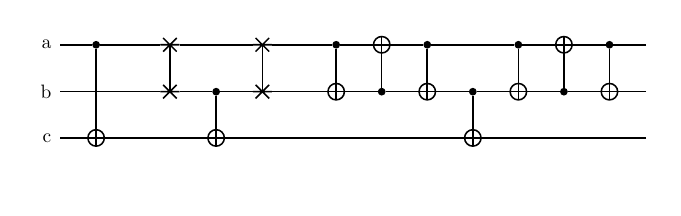
\begin{tikzpicture}
\node[scale=0.7] {
  \begin{quantikz}
  \lstick{a} & \ctrl{2} & \qw \qceq & \swap{1} & \qw & \swap{1} & \qw\qceq & \ctrl{1} & \targ{} & \ctrl{1} & \qw &\ctrl{1} & \targ{} & \ctrl{1} & \qw \\
  \lstick{b} & \qw & \qw & \swap{} & \ctrl{1} & \swap{} & \qw & \targ{} & \ctrl{-1}& \targ{} & \ctrl{1} & \targ{} & \ctrl{-1}& \targ{} & \qw \\
  \lstick{c} & \targ{} & \qw  & \qw & \targ{} & \qw & \qw & \qw & \qw & \qw & \targ & \qw & \qw & \qw & \qw  & \qw \\
  \end{quantikz}
};
\end{tikzpicture}
  \caption{Applying a CNOT gate on $(a, c)$ using a SWAP gate}
\end{figure}

\begin{figure}[h]
  \label{fig:bridge-one-with-bridge}
  \centering
  \begin{quantikz}
  \lstick{a} & \ctrl{2} & \qw \qceq & \qw & \ctrl{1} & \qw & \ctrl{1} & \qw \\
  \lstick{b} & \qw & \qw & \ctrl{1} & \targ{} & \ctrl{1}  & \targ{} & \qw \\
  \lstick{c} & \targ{} & \qw & \targ{} & \qw  & \targ & \qw  & \qw &  \qw \\
  \end{quantikz}
  \caption{Applying a CNOT gate on $(a, c)$ using a bridge gate}
\end{figure}

Figure~\ref{fig:bridge-one-with-swap} and \ref{fig:bridge-one-with-bridge} show the difference between using a SWAP gate and a bridge gate to perform a CNOT gate for the case of three qubits. The bridge gate is more efficient in terms of the number of CNOT gates, but it is less efficient in terms of depth.

Now, the generalized bridge gate is defined as follows~\cite{nash2020}:

\begin{definition}{Generalized Bridge Gate}
  A CNOT between qubit $1$ and $n$ can be performed using a generalized bridge gate as follows:
  \begin{equation} \mathrm{Bridge}(1, n) = \prod_{i=1}^{n - 1}(\mathrm{CNOT}(i + 1, i) \prod_{i=n - 2}^{2}\mathrm{CNOT}(i + 1, i))^2
  \end{equation}
\end{definition}


\def\qceq{\midstick[6,brackets=none]{=}}
\begin{figure}[h]
  \centering
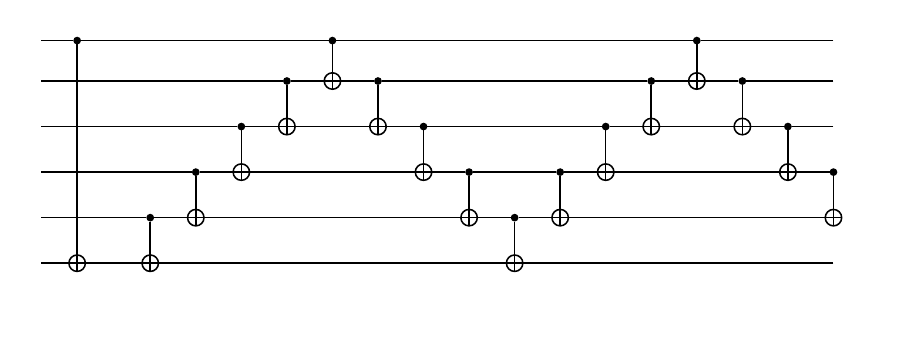
\begin{tikzpicture}
\node[scale=0.7] {
\begin{quantikz}
\qw &\ctrl{5}&\qw\qceq&
 \qw    &\qw     &\qw     &\qw     &\ctrl{1}& \qw    & \qw    & \qw     &
 \qw    &\qw     &\qw     &\qw     &\ctrl{1}& \qw    & \qw    & \qw     & \\
\qw & \qw    & \qw    &
 \qw    &\qw     &\qw     &\ctrl{1}& \targ{}&\ctrl{1}& \qw    & \qw     &
 \qw    &\qw     &\qw     &\ctrl{1}& \targ{}&\ctrl{1}& \qw    & \qw     & \\
\qw & \qw    & \qw    &
 \qw    &\qw     &\ctrl{1}& \targ{}& \qw    &\targ{} &\ctrl{1}& \qw     &
 \qw    &\qw     &\ctrl{1}& \targ{}& \qw    &\targ{} &\ctrl{1}& \qw     & \\
\qw & \qw    & \qw    &
 \qw    &\ctrl{1}&\targ{} & \qw    & \qw    & \qw    &\targ{} &\ctrl{1} &
 \qw    &\ctrl{1}&\targ{} & \qw    & \qw    & \qw    &\targ{} &\ctrl{1} & \\
\qw & \qw    & \qw    &
\ctrl{1}&\targ{} &\qw     & \qw    & \qw    & \qw    & \qw    &\targ{}  &
\ctrl{1}&\targ{} &\qw     & \qw    & \qw    & \qw    & \qw    &\targ{}  & \\
\qw &\targ{} & \qw    &
\targ{} & \qw    & \qw    & \qw    & \qw    & \qw    & \qw     & \qw    &
\targ{} & \qw    & \qw    & \qw    & \qw    & \qw    & \qw     & \qw    & \\
\end{quantikz}
};
\end{tikzpicture}
  \caption{The bridge gate for $n=6$}
\end{figure}

\subsection{Circuit Optimization}

Circuit optimization is often achieved by applying simplification rules to the circuit~\cite{pointing2021}. These simplification rules are usually based on the commutation relations of the gates~\cite{itoko2019}.

Yet, this simplification rules are implemented as a pattern matching, therefore the hidden patterns that can be revealed by another simplification rules will not be found.

\section{Hamiltonian Compilation}

The literature on Hamiltonian compilation is currently limited. Even existing compilers have not implemented anything beyond a first-order Suzuki-Trotter decomposition~\cite{sivarajah2021, qiskit2023}. Also, if we consider the Suzuki-Trotter decomposition as a compiler, there are also a few related works that could be considered as a part of the literature, such as an analysis of its error~\cite{childs2021}.

Not all efforts in Hamiltonian compilation are based on the Suzuki-Trotter decomposition. Another approach is to use a randomized compiler based on sampling Hamiltonian terms~\cite{campbell2019}. This method is called QDRIFT protocol and it is briefly described in the theorem below.

\begin{theorem}[QDRIFT Compiler]
  Given $H = \sum_{j=1}^k h_j$ and an oracle that samples the terms of the Hamiltonian by weight $\frac{\norm{h_i}_\infty}{\sum_{j=1}^k \norm{h_j}_\infty}$, by randomly sampling $N$ terms $\eta_1 \dots \eta_N$, then we can define the approximate evolution as
  \begin{equation}
    U(t) = \prod_{i=1}^N e^{it\frac{\eta}{N}\sum_{j=1}^k \norm{h_j}_\infty}
  \end{equation}
  where it asymptotically outperform first-order Suzuki-Trotter decomposition in number of gates at a certain level of error.
\end{theorem}

Our baseline compiler is described in~\cite{lao2021}, which uses the Suzuki-Trotter decomposition and defines routing and scheduling algorithms specifically for Hamiltonian compilation.

The compiler includes two different heuristic search algorithms, one for initial qubit allocation and another for subsequent qubit allocation. The algorithm for subsequent qubit allocation also provides the route (of SWAP gates) for reallocation. This compiler supports all one and two-qubit gates as intermediate gates, which helps simplify the circuit by unifying consecutive two-qubit gates~\cite{lao2021}.


\subsection{Scheduling}

Even general quantum circuits may have a small degree of freedom in the order of execution. Moreover, the approximate circuit of a Hamiltonian may have a total arbitrariness in the order of execution. This degree of freedom can be set wisely to reduce the complexity of the circuit.

\begin{problem}[Scheduling]
  Given a quantum circuit that has a DAG of dependencies, the scheduling problem seeks for an optimal order of execution of the gates.
\end{problem}

Several heuristic algorithms have been proposed in the literature for both Hamiltonians~\cite{lao2021} and the general case~\cite{zhou2020, zulehner2018}.

\chapter{Open Problems and Related Questions}\label{chap:open_problems}

We encountered several open problems and related questions while working on Hamiltonian compilation, which are listed below along with brief notes on our thoughts about them.

\begin{itemize}
  \item \textbf{Optimality of Bridge Gates}: It has been shown that the bridge gate for $n$ qubits has a depth and number of CNOT gates of $4n + O(1)$. This is equivalent to $3n + O(1)$ and $6n + O(1)$, respectively, for the naive SWAP gates, indicating that one of them is better in terms of depth and the other outperforms in the number of CNOT gates.

  We have already shown that there is another design for bridge gates with $4n + O(1)$ and $n + O(1)$, and furthermore, it is optimal.

  \item \textbf{Bridging Other Two-Qubit Gates}: The bridge gate is currently only defined for CNOT gates. The question is whether it is possible to define a bridge gate for all two-qubit gates.
  
  We have shown that there is a SWAP bridge gate for three qubits that requires $8$ CNOT gates, rather than the naive $9$ CNOT gates. Surprisingly, it could not be generalized, and the naive SWAPs are asymptotically optimal.

  \item \textbf{Defining Problems on Hamiltonian Graph}: We already know that a device graph, due to the restrictions imposed by the physical hardware, is not much like an arbitrary graph and could be represented by simpler structures than graphs (like indices of the lattice, etc.). For the compilation of Hamiltonians, we also have another graph, the Hamiltonian graph, which is a hypergraph with a hyperedge for each Hamiltonian term. If we can define the problems on the Hamiltonian graph rather than the device graph, it may be easier to solve them. 

  Currently, we are working on Hamiltonian graph coloring as a way to group the gates of Suzuki-Trotter decomposition into layers. We are hopeful that this approach will help solve 
  allocation and scheduling subproblems.

  Moreover, after defining explicit layers, then the scheduling problem can be seen as a variant of traveling salesman problem, which is a well-studied problem in the literature.
\end{itemize}
\chapter{Conclusion}\label{chap:conclusion}

In conclusion, quantum compilation is a crucial step towards the realization of useful quantum computations on noisy and intermediate-scale devices. In this essay, we have started with the important tools that are necessary for designing and implmentation of a Hamiltonian compiler. We have also reviewed some of the recent advancements in quantum compilation, in general and Hamiltonian compilation as well. Finally discussed some of the open problems and related questions in the field. We believe that addressing these open problems will help us to improve the performance of the Hamiltonian compilers.

\printbibliography

\end{document}

